\section{The \textbf{TransP-0} design space}
%\section{The \textbf{TransP-0} integrated design abstraction}
\label{proposed_model}

The \textsc{TransP-0} design framework is intended to support both transportation and power system engineers
during early project phases 
in formulating and evaluating different design options quickly. Therefore, transportation and energy system properties - both static and dynamic - have to be captured sufficiently precise. On the other hand, the design abstraction should omit unnecessary details to enable frequent design iterations. With these requirements in mind we have developed a candidate design abstraction, which is summarized in Figure~\ref{system_design}. The abstraction comprises various transportation and energy subsystem parameters. Note that we have tried to reduce the number of parameters to a minimum, taking potentially decreased physical accuracy into account.

\begin{figure}[h!]
	\begin{center}
	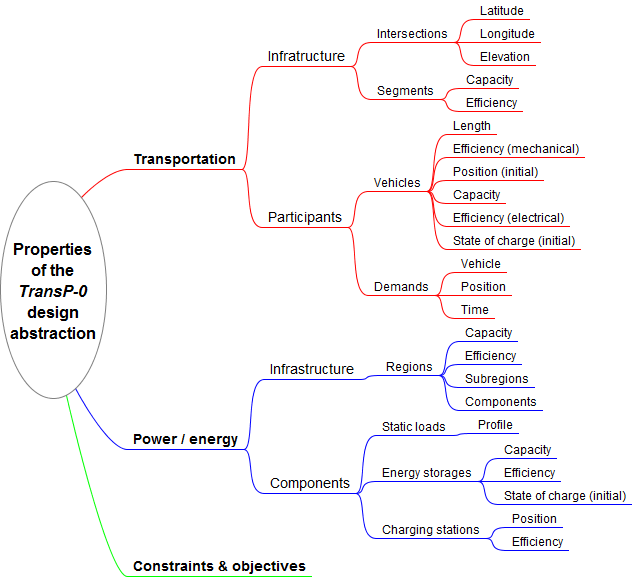
\includegraphics[trim=0 10 0 0, width=0.875\columnwidth]{./gfx/system_design.png}
	\caption{Overview over the \textsc{TransP-0} design space parameters comprising the transportation and the energy subsystem.}
	\label{system_design}
	\end{center}
\end{figure}

Subsequently we describe the design space parameters for the transportation subsystem in Section~\ref{transport} and the energy subsystem in Section~\ref{energy_system}.

\subsection{Transportation subsystem}
\label{transport}

We decided to model the transportation subsystem in a mesoscopic fashion~\cite{?}. In particular, our model includes a representation of the road network and each individual vehicle. The road network is modeled as a directed graph, where nodes represent intersections and edges represent road segments. Hereby, the edge weight defines the number of lanes and the edge direction indicates the intended driving direction. Consequently, two edges have to be used to describe bidirectional traffic flows. 
%Here, the vehicles represent ''particles'' that are traveling along the road network. 
Vehicles are assigned to points on the edges of the road network. Hence, vehicles are able to move along edges and jump between edges at intersections. The \textsc{TransP-0} abstraction of the transportation subsystem is illustrated in Figure~\ref{transport_illustration}.

\begin{figure}[h]
	\begin{center}
	\includegraphics[trim=0 6 0 21, width=.825\columnwidth]{./gfx/transportation_system2.png}
	\caption{Illustration of a transportation subsystem design including an infrastructure (composed of road intersections (red) and segments (grey)) and participants (green).}
	\label{transport_illustration}
	\end{center}
\end{figure}

Formally, the transportation subsystem $TS$ of the integrated design abstraction is modeled as a tuple $(TSI, TSP)$, where
\begin{itemize}
	\item $TSI$ represents the \textit{transportation infrastructure} (i.e.\ roads and their intersections) and
	\item $TSP$ represents the individual \textit{traffic participants} (i.e.\ passenger cars and goods vehicles).
\end{itemize}
Essentially, we distinguish between the static (i.e.\ the infrastructure) and the dynamic (i.e.\ the participants) parts of the transportation subsystem. In the following, we describe the the infrastructure design abstraction in Section~\ref{transport_infrastructure} before explaining the participant design abstraction in Section~\ref{participants}.

\subsubsection{Infrastructure}
\label{transport_infrastructure}

The transportation subsystem infrastructure $TSI$ of the transportation subsystem $TS$ is modeled as a tuple $(RI, RS)$, where
\begin{itemize}
	\item $RI$ represents \textit{road intersections} (i.e.\ the points in geometric space where roads intersect) and
	\item $RS$ represent {road segments} (i.e.\ the actual roads leading from intersection to intersection).
\end{itemize}
Road intersections and segments make up a directed graph describing the transportation subsystem infrastructure. Subsequently, we first describe road intersections in Section~\ref{intersections} before explaining road segments in Section~\ref{segments}.

\paragraph{Intersections}
\label{intersections}

The road intersections $RI$ of the transportation subsystem infrastructure $TSI$ are modeled - again - as a tuple $(RIL, RIC)$, where
\begin{itemize}
	\item $RIL$ represents a finite set of road intersection \textit{labels} and
	\item $RIC: RIL \rightarrow \mathbb{R}^3$ represents a mapping from road intersection labels to geometric coordinates.
\end{itemize}
Note that typically the coordinates are expressed in terms of latitude, longitude, and elevation. However, for simplicity in this work we use Cartesian coordinates instead. Consequently, distances can be computed more easily using the Euclidean metric. 
%Moreover, transformations exist to switch between polar and Cartesian coordinates.

\paragraph{Segments}
\label{segments}

The road segments $RS$ of the transportation subsystem infrastructure $TSI$ are modeled as a five-tuple $(RSL, RSS, RST, RSC, RSE)$, where
\begin{itemize}
	\item $RSL$ represents a finite set of road segment \textit{labels},
	\item $RSS/RST: RSL \rightarrow RIL$ represent mappings from road segment labels to their respective \textit{source} and \textit{target} road intersection labels,
	\item $RSC: RSL \rightarrow \mathbb{N}$ represents a mapping from road segment labels to their \textit{capacities} (i.e.\ the number of lanes of the road segment), and
	\item $RSE: RSL \rightarrow \mathbb{R}^+$ represents a mapping from road segment labels to their \textit{efficiency} (i.e.\ surface material of the road segment).
\end{itemize}
Note that the previous parameters completely determine our road segment model. Consequently, we abstract from a variety of parameters typically considered such as continuous elevation profiles~\cite{?} or surface friction coefficients~\cite{?}.

Furthermore, we derive the road segment distance $RSD: RSL \rightarrow \mathbb{R}_0^+$ as a mapping from road segment labels to distances and we use the Euclidean metric $E: \mathbb{R}^3 \times \mathbb{R}^3 \rightarrow \mathbb{R}_0^+$ to compute the road segment distance as
\[
	RSD(rsl) = E(RIC(RSS(rsl)), RIC(RST(rsl))) \textrm{.}
\]
Finally, we define road segment positions $RSP \subseteq RSL \times \mathbb{R}_0^+$ as tuples of road segment labels and traveled distances
\[
	RSP = \{(rsl, d) \in RSL \times \mathbb{R}_0^+ \mid d \leq RSD(rsl)\} \textrm{.}
\]
We use the road segment positions $RSP$ to locate traffic participants (i.e.\ vehicles) on the transportation subsystem infrastructure $TSI$ as explained in Section~\ref{participants}. 
%Note that the world coordinates can be obtained by a respective coordinate transformation.

\subsubsection{Participants}
\label{participants}

The transportation subsystem participants $TSP$ of the transportation subsystem $TS$ are modeled as a tuple $(V, D)$, where
\begin{itemize}
	\item $V$ represents the vehicles (i.e.\ the physical objects using the transportation subsystem infrastructure) and
	\item $D$ represents the demands (i.e.\ the logical objects that cause the movement of the physical objects).
\end{itemize}
Consequently, we - again - distinguish between the static (i.e.\ the vehicles) and the dynamic (i.e.\ the demands) parts of the model. In the following, we first describe the vehicle design abstraction in Section~\ref{vehicles} before explaining the demand design abstraction in Section~\ref{demands}.

\paragraph{Vehicles}
\label{vehicles}

The vehicles $V$ of the transportation subsystem participants $TSP$ are modeled as seven-tuple $(VL, VS, VME, VP_0, VC, VEE, VSOC_0)$, where
\begin{itemize}
	\item $VL$ represents a finite set of vehicle \textit{labels},
	\item $VS: VL \rightarrow \mathbb{R}^+$ represents a mapping from vehicle labels to their \textit{size} (i.e.\ the length of the vehicle in road segment direction),
	\item $VME: VL \rightarrow \mathbb{R}^+$ represents a mapping from vehicle labels to their \textit{mechanical efficiency} (i.e.\ a constant ratio for the conversion between electrical and mechanical energy),
	\item $VP_0: VL \rightarrow RSP$ represents a mapping from vehicle labels to their initial road segment \textit{positions} (see Section~\ref{segments}),
	\item $VC: VL \rightarrow \mathbb{R}^+$ represents a mapping from vehicle labels to their battery \textit{capacities} (i.e.\ the maximum amount of energy that can be stored by the vehicle),
	\item $VEE: VL \rightarrow \mathbb{R}^+$ represents a mapping from vehicle labels to their \textit{electrical efficiency} (i.e.\ a constant ratio for conversion between electrical energy and stored energy), and
	\item $VSOC_0: VL \rightarrow \mathbb{R}^+$ represents a mapping from vehicle labels to their initial \textit{state of charge} (i.e.\ the amount of energy stored by the vehicle initially) such that
	\[
		\forall vl \in VL : VSOC_0(vl) \leq VC(vl) \textrm{.}
	\]
\end{itemize}
Note that we again abstract from many parameters typically considered such as vehicle weight~\cite{?} or exact vehicle geometry~\cite{?}. In particular, we approximate mechanical and electrical efficiencies with constants only.

\paragraph{Demands}
\label{demands}

Finally, the demands $D$ of the transportation subsystem participants $TSP$ are modeled as four-tuple $(DL, DV, DP, DT)$, where
\begin{itemize}
	\item $DL$ represents a finite set of demand \textit{labels},
	\item $DV: DL \rightarrow VL$ represents a mapping from demand labels to \textit{vehicle} labels (i.e.\ the concerned vehicle),
	\item $DP: DL \rightarrow RSP$ represents a mapping from demand labels to road segment \textit{positions} (i.e.\ where the concerned vehicle is expected to be), and
	\item $DT: DL \rightarrow \mathbb{N}^+$ represents a mapping from demand labels to \textit{time} points (i.e.\ when the concerned vehicle is expected to be there)
\end{itemize}
Note that our abstraction is based on discrete time. However, we do not prescribe the time step resolution. For long travel distances and durations more coarse resolutions can be used, for shorted distances and durations more fine-grained resolutions are needed typically.

\subsection{Power / energy subsystem}
\label{energy_system}

Similar to the transportation subsystem (see Section~\ref{transport}), we decided to model the energy subsystem in a mesoscopic fashion~\cite{Hackenberg2012}. Note that microscopic models represent the individual power lines and their physical characteristics~\cite{Dommel1968}, while macroscopic models aggregate the entire energy subsystem into a single marketplace without power line characteristics~\cite{Castronuovo2004}. Our mesoscopic model takes an intermediate approach, where only selected characteristics of the power line topology are represented. In particular, we limit our representation to subnetworks of equal voltage level (i.e.\ the \textit{network regions}) and their hierarchical connectivity. Consequently, balances can be computed also for single regions rather than the entire electricity market. Finally, the \textsc{TransP-0} abstraction of the energy subsystem is illustrated in Figure~\ref{energy_illustration}.

\begin{figure}[h]
	\begin{center}
	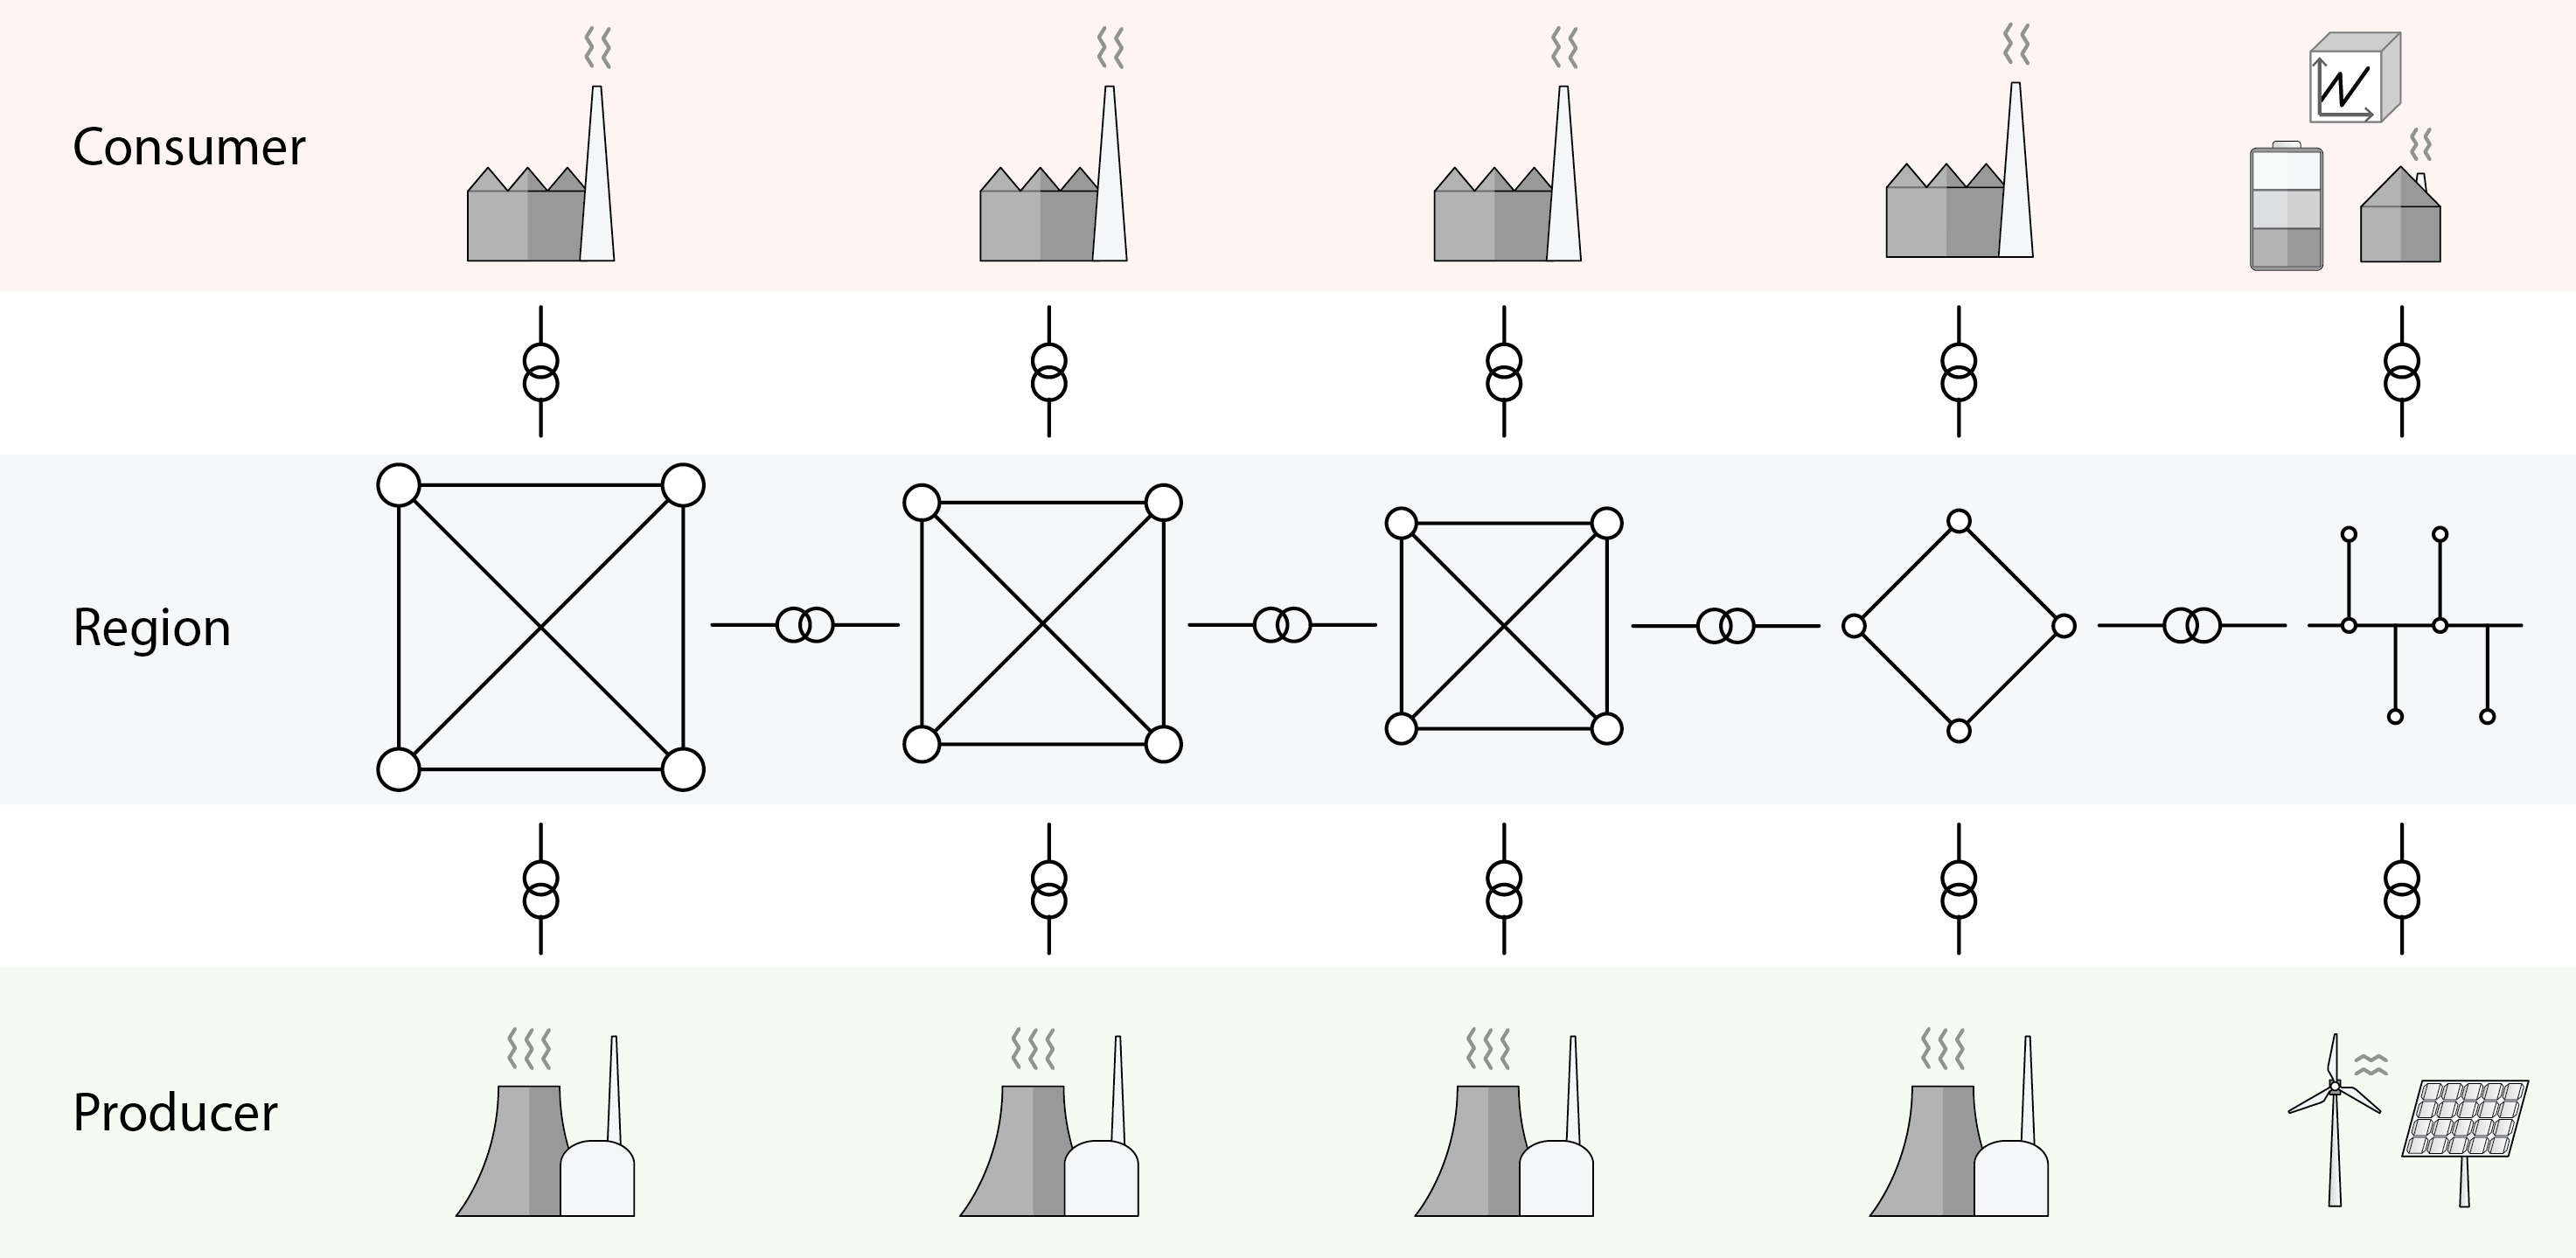
\includegraphics[trim=0 10 0 15, width=0.95\columnwidth]{./gfx/energy_system.png}
	\caption{Illustration of a energy subsystem design including an infrastructure (composed of regions) and components (i.e.\ producers and consumers).}
	\label{energy_illustration}
	\end{center}
\end{figure}

Formally, the energy subsystem $ES$ of the integrated design abstraction is modeled as a tuple $(ESI, ESC)$, where
\begin{itemize}
	\item $ESI$ represents the \textit{energy subsystem infrastructure} (i.e.\ the transmission and distribution network) and
	\item $ESC$ represents \textit{energy subsystem components} (i.e.\ the actual producers and consumers).
\end{itemize}
Hence, we separate network characteristics and network usage. Subsequently, we first explain the infrastructure in Section~\ref{regions} before describing the components in Section~\ref{components}.

\subsubsection{Infrastructure}
\label{energy_infrastructure}

The energy subsystem infrastructure $ESI$ of the energy subsystem $ES$ is modeled as a one-tuple $(R)$, where
\begin{itemize}
	\item $R$ represents the \textit{regions} of the energy subsystem infrastructure, which are determined by the voltage levels and transformers of the network.
\end{itemize}
Note that we selected a region model~\cite{Hackenberg2012} over a power flow model~\cite{Dommel1968} to reduce modeling effort and increase computational efficiency. In the following, we describe the regions in Section~\ref{regions}.

\paragraph{Regions}
\label{regions}

The network regions $R$ of the energy subsystem infrastructure $ESI$ are modeled as a four-tuple $(RL, RC, RE, RP)$, where
\begin{itemize}
	\item $RL$ represents a finite set of region labels,
	\item $RC: RL \rightarrow \mathbb{R}^+$ represents a mapping from region labels to their \textit{capacities} (i.e.\ the maximum amount of energy that can flow through each region in a predefined time interval),
	\item $RE: RL \rightarrow \mathbb{R}^+$ represents a mapping from region labels to region \textit{efficiencies} (i.e.\ a constant factor determining the energy that is lost while flowing through that region), and
	\item $RP: RL \rightarrow RP \cup \{\bot\}$ represents a mapping from region labels to their \textit{parent} region label (i.e.\ the superordinate voltage level or the start symbol $\bot$).
\end{itemize}
Note that regions must be assigned to at most one parent region. Consequently, our region model represents the energy system as a tree structure. The nodes of the tree represent \textit{subnetworks} with distinct voltage levels. The edges of the tree represent \textit{transformers} connecting the subnetworks instead. The region model can be derived from existing network topologies easily.

\subsubsection{Components}
\label{components}

The energy subsystem components $ESC$ of the energy subsystem $ES$ is modeled as a three-tuple $(SL, ES, CS)$, where
\begin{itemize}
	\item $SL$ represents the \textit{static loads} (i.e.\ loads assumed to be uncontrollable in our approach),
	\item $ES$ represents the stationary \textit{energy storages} (i.e.\ variable producers and consumers), and
	\item $CS$ represents the \textit{charging stations} for the electric vehicles (see Section~\ref{vehicles}).
\end{itemize}
In the following, we first explain the static load design abstraction in Section~\ref{static_loads}, before describing the energy storage design abstraction in Section~\ref{energy_storages} and presenting the charging station design abstraction in Section~\ref{charging_stations}.

\paragraph{Static loads}
\label{static_loads}

The static loads $SL$ of the energy subsystem components $ESC$ are modeled as three-tuple $(SLL, SLP, SLR)$, where
\begin{itemize}
	\item $SLL$ represents a finite set of static load \textit{labels},
	\item $SLP: SLL \rightarrow (\mathbb{N} \rightarrow \mathbb{R})$ represents a mapping from static load labels $SLL$ to static load \textit{profiles} (i.e.\ a predefined production and consumption curve), and
	\item $SLR: SLL \rightarrow RL$ represents a mapping from static load labels to parent \textit{region} labels (i.e.\ the region where the static load is attached).
\end{itemize}
Note that static load profiles associate a numeric load to each discrete time step. Hereby positive loads represent energy production and negative loads represent energy consumption. Consequently, static loads can be used to model everything from home appliances over solar panels to conventional power generators. In particular, we assume such loads to be uncontrollable in our design abstraction and the perspective of the system engineer.

\paragraph{Energy storages}
\label{energy_storages}

Then, the energy storages $ES$ of the energy subsystem components $ESC$ are modeled as a five-tuple $(ESL, ESCA, ESE, ESS_0, ESR)$, where
\begin{itemize}
	\item $ESL$ represent a finite set of energy storage \textit{labels},
	\item $ESCA: ESL \rightarrow \mathbb{R}^+$ represents a mapping from energy storage labels to energy storage \textit{capacities} (i.e.\ the maximum amount of energy that can be stored),
	\item $ESE: ESL \rightarrow \mathbb{R}^+$ represents a mapping from energy storage labels to energy storage \textit{efficiencies} (i.e.\ a constant factor between inflowing energy and stored energy), and
	\item $ESS_0: ESL \rightarrow \mathbb{R}_0^+$ represents a mapping from energy storage labels to initial \textit{state of charges} (i.e.\ the amount of energy stored initially) such that
	\[
		ESS_0(esl) \leq ESCA(esl) \textrm{, and}
	\]
	\item $ESR: ESL \rightarrow RL$ represents a mapping from energy storage labels to parent \textit{region} labels (i.e.\ the region where the energy storage is attached).
\end{itemize}
Note that the energy storage model is analogous to the electric vehicle model present in Section~\ref{vehicles}. However, electric vehicles additionally define mechanical parameters, while energy storages are attached to regions statically. Furthermore, we currently target small batteries rather than large storage facilities. Larger facilities require more parameters instead.

\paragraph{Charging stations}
\label{charging_stations}

Finally, the charging stations $CS$ of the energy subsystem components $ESC$ are modeled as a four-tuple $(CSL, CSP, CSE, CSR)$, where
\begin{itemize}
	\item $CSL$ represents a finite set of charging station \textit{labels},
	\item $CSE: CSL \rightarrow \mathbb{R}^+$ represents a mapping from charging station labels to charging station \textit{efficiencies} (i.e.\ a loss factor for respective energy flows), and
	\item $CSP: CSL \rightarrow RSL$ represents a mapping from charging station labels to road segment labels with zero road segment distance, i.e.\
	\[
		RSD(CSP(csl)) = 0 \textrm{, and}
	\]
	\item $CSR: CSL \rightarrow RL$ represents a mapping from charging station labels to parent \textit{region} labels (i.e.\ the region where the charging station is attached).
\end{itemize}
Note that the charging station position mapping $CSP$  and the charging station region mapping $CSR$ define the static connections between the transportation subsystem and the energy subsystem. Consequently, vehicles (see Section~\ref{vehicles}) are able to interact with arbitrary regions (see Section~\ref{regions}) of the energy subsystem infrastructure at predefined zero-length road segments (see Section~\ref{segments}).
